\subsection{Implementation}
We implement a framework in order  to simplify parameter estimation for 
pulse-chase RNA-seq experiments. 
We use \emph{R} programming environment, 
because it allows very flexible handling of user-specified models, 
includes implementations a variety of commonly used procedures and 
has powerfull plotting features \citep{rlang}.
\par A user needs to provide
\begin{itemize}
 \item a count table with the raw read numbers
 \item a condition matrix (to infer sample fractions in the count table)
 \item formulas for the mean read numbers, e.g. 
 $r_\text{L}\sim \mu e^{-dt}$, (section~\ref{subsec:kinetics}).
 \item spike-ins, if relevant
\end{itemize}
The package utilizes so-called \emph{non-standard evaluation},
a feature of the \emph{R} language \citep{team2000r}.
This allows to handle arbitrary formulas, which the user supplies for 
the mean gene expression levels. Hence, no manual 
implementation for the likelihood functions is necessary and the 
formulas are needed to defined only once.
\subsection{Evaluation on simulated data}
To demonstrate the analysis workflow, we generated a data 
set on the basis of the pulse-model, introduced in the section~2.
\begin{align}
 r_\text{i,T}&=\mu_i\\
 r_\text{i,L}&=\mu_i \left(1-e^{-d_it_\text{L}}\right)\\
 r_\text{i,U}&=\mu_i e^{-d_it_\text{L}},
\end{align}
where $t_\text{L} = 12$ hr is the time amount of pulse-labelling,
$i \in 1..100$ is a gene index, $\mu_i$ and $d_i$ are gene-specific parameters,
which are sampled from random number generator.
Usually concentration of RNA in the samples is normalised before the
sequencing procedure \citep{}. This introduces a bias, which 
we model by fraction coefficients in section~\ref{subsec:normalisation}. 
For the data set we 

\begin{figure}
 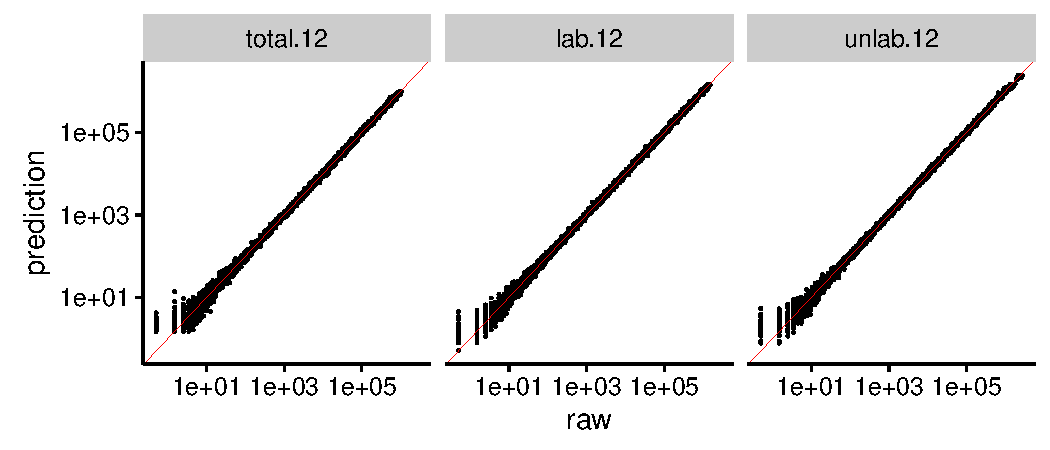
\includegraphics[width=\linewidth]{fig/predictions}
 \caption{Model predictions.}
\end{figure}

\begin{figure}
 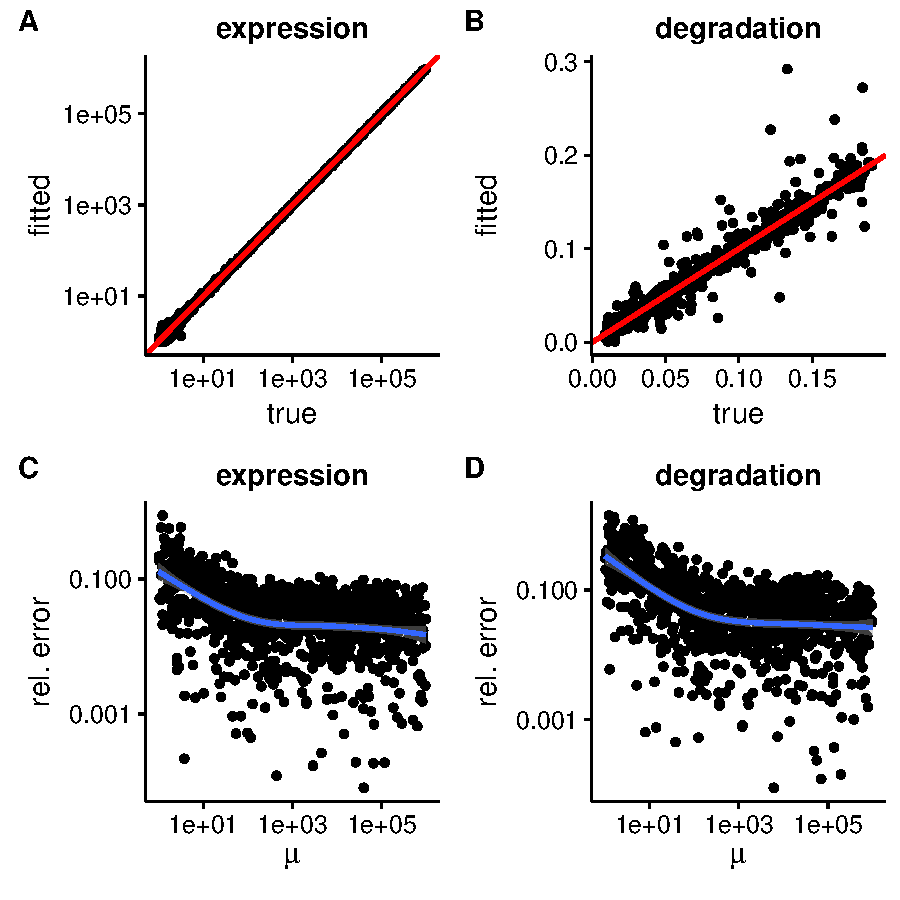
\includegraphics[width=\linewidth]{fig/parameters}\\
 \caption{Parameter misprediction.}
\end{figure}